\ifdefined\inMainDoc\else
\documentclass[12pt,a4paper]{article}
% ================================================================
%  PRÉAMBULE COMMUN - ANNALES CORRIGÉES
%  Université de Kara - FaST - Licence Fondamentale MPC
%  Design optimisé impression noir et blanc
% ================================================================

% -- ENCODAGE & LANGUE --
\usepackage[utf8]{inputenc}
\usepackage[T1]{fontenc}
\usepackage[french]{babel}
\usepackage{lmodern}
\usepackage{microtype}

% -- MISE EN PAGE --
\usepackage[a4paper, top=2.8cm, bottom=2.5cm, left=2.5cm, right=2.5cm, headheight=14pt]{geometry}
\usepackage{setspace}
\setstretch{1.2}
\usepackage{parskip}
\setlength{\parindent}{1.2em}
\setlength{\parskip}{4pt}

% -- MATHS --
\usepackage{amsmath, amssymb, mathtools, amsthm}
\usepackage{mathrsfs}
\usepackage{dsfont}
\usepackage{bm}
\usepackage{cancel}
\usepackage{textcomp}
% Définition de \oiint (intégrale de surface fermée) sans package supplémentaire
\newcommand{\oiint}{\mathop{\iint\!\!\!\!\!\!\!\bigcirc}\limits}

% -- PHYSIQUE & CHIMIE --
\usepackage{physics}
\usepackage{siunitx}
% Lorsque physics est chargé, siunitx omet \qty. On le restaure ici :
\AtBeginDocument{\RenewCommandCopy\qty\SI}
\sisetup{locale = FR, detect-all, output-decimal-marker={,}}
% Commande de substitution pour les unités posant problème avec pdflatex
% (ohm, degreeCelsius, micro, angstrom, percent utilisent des caractères non-ASCII)
\newcommand{\qtyohm}[1]{\ensuremath{\num{#1}\,\Omega}}
\newcommand{\qtydegc}[1]{\ensuremath{\num{#1}\,{}^\circ\text{C}}}
\newcommand{\qtyangstrom}[1]{\ensuremath{\num{#1}\,\text{\AA}}}
\newcommand{\qtypercent}[1]{\ensuremath{\num{#1}\,\%}}
\newcommand{\qtyum}[1]{\ensuremath{\num{#1}\,\mu\text{m}}}
\usepackage[version=4]{mhchem}

% -- GRAPHISMES --
\usepackage{graphicx}
\usepackage{float}
\usepackage{caption}
\usepackage{subcaption}
\usepackage{wrapfig}
\usepackage{tikz}
\usetikzlibrary{calc, arrows.meta, patterns, shapes.geometric}
\usepackage{pgfplots}
\pgfplotsset{compat=1.18}

% -- TABLEAUX --
\usepackage{booktabs}
\usepackage{array}
\usepackage{tabularx}
\usepackage{multirow}

% -- LISTES --
\usepackage{enumitem}
\setlist[enumerate]{topsep=3pt, itemsep=2pt, parsep=0pt}
\setlist[itemize]{topsep=3pt, itemsep=2pt, parsep=0pt, label={.}}

% -- BOÎTES (noir et blanc) --
\usepackage{mdframed}
\usepackage{tcolorbox}
\tcbuselibrary{skins, breakable, theorems}

% Boîte EXERCICE : encadré avec filet épais, fond blanc
\newmdenv[
  linewidth=1.2pt,
  linecolor=black,
  roundcorner=3pt,
  skipabove=10pt,
  skipbelow=6pt,
  innertopmargin=8pt,
  innerbottommargin=8pt,
  innerleftmargin=10pt,
  innerrightmargin=10pt,
  backgroundcolor=white,
  frametitle={\bfseries\small Exercice},
  frametitlealignment=\raggedright,
  frametitleaboveskip=4pt,
  frametitlebelowskip=4pt,
]{boiteexercice}

% Boîte CORRIGÉ : fond gris très clair + filet fin
\newmdenv[
  linewidth=0.6pt,
  linecolor=black,
  leftline=true,
  rightline=false,
  topline=false,
  bottomline=false,
  linecolor=black,
  innerleftmargin=12pt,
  innerrightmargin=8pt,
  innertopmargin=6pt,
  innerbottommargin=6pt,
  backgroundcolor=gray!8,
  skipabove=4pt,
  skipbelow=8pt,
]{boitecorrige}

% Boîte RÉSUMÉ DE COURS : double encadré
\newmdenv[
  linewidth=0.8pt,
  linecolor=black,
  roundcorner=2pt,
  backgroundcolor=gray!12,
  innertopmargin=10pt,
  innerbottommargin=10pt,
  innerleftmargin=12pt,
  innerrightmargin=12pt,
  skipabove=12pt,
  skipbelow=8pt,
]{boiteresume}

% Boîte ATTENTION/REMARQUE : barre gauche épaisse
\newmdenv[
  leftline=true,
  rightline=false,
  topline=false,
  bottomline=false,
  linewidth=3pt,
  linecolor=black,
  backgroundcolor=gray!5,
  innerleftmargin=12pt,
  innerrightmargin=8pt,
  innertopmargin=5pt,
  innerbottommargin=5pt,
  skipabove=6pt,
  skipbelow=6pt,
]{boiteremarque}

% -- DIFFICULTÉ DES EXERCICES --
\newcommand{\facile}{$\star$}
\newcommand{\moyen}{$\star\!\star$}
\newcommand{\difficile}{$\star\!\star\!\star$}
\newcommand{\niveau}[1]{\hfill\textbf{#1}\hspace{2pt}}

% -- EN-TÊTES ET PIEDS DE PAGE --
\usepackage{fancyhdr}
\pagestyle{fancy}
\fancyhf{}
\renewcommand{\headrulewidth}{0.5pt}
\renewcommand{\footrulewidth}{0.3pt}

% -- HYPERLIENS --
\usepackage[hidelinks]{hyperref}
\hypersetup{
    colorlinks=false,
    pdftitle={Annale Corrigée - Licence MPC - Université de Kara}
}

% -- TITRES --
\usepackage{titlesec}
\titleformat{\section}{\Large\bfseries}{\thesection.}{0.8em}{}[\vspace{2pt}\hrule\vspace{4pt}]
\titleformat{\subsection}{\large\bfseries}{\thesubsection.}{0.7em}{}
\titleformat{\subsubsection}{\normalsize\bfseries}{\thesubsubsection.}{0.6em}{}

% -- THÉORÈMES --
\theoremstyle{definition}
\newtheorem{defn}{Définition}[section]
\newtheorem{prop}{Propriété}[section]
\newtheorem{thm}{Théorème}[section]
\newtheorem{corol}{Corollaire}[section]
\newtheorem{exemple}{Exemple}[section]

% -- COMMANDES MATHÉMATIQUES UTILES --
\newcommand{\vect}[1]{\overrightarrow{#1}}
\newcommand{\R}{\mathbb{R}}
\newcommand{\N}{\mathbb{N}}
\newcommand{\Z}{\mathbb{Z}}
\newcommand{\C}{\mathbb{C}}
\renewcommand{\d}{\mathrm{d}}
\newcommand{\deriv}[2]{\dfrac{\d #1}{\d #2}}
\newcommand{\dpart}[2]{\dfrac{\partial #1}{\partial #2}}
\newcommand{\rot}{\overrightarrow{\mathrm{rot}}\,}
\renewcommand{\div}{\mathrm{div}\,}
\renewcommand{\grad}{\overrightarrow{\mathrm{grad}}\,}
\newcommand{\e}{\mathrm{e}}
\newcommand{\ii}{\mathrm{i}}
\renewcommand{\Tr}{\mathrm{Tr}}

% Numérotation des équations par section
\numberwithin{equation}{section}

% -- RÉSULTATS ENCADRÉS --
\newcommand{\res}[1]{\[\boxed{#1}\]}

% -- REMARQUE INLINE --
\newcommand{\rmq}[1]{\begin{boiteremarque}\textbf{Remarque.} #1\end{boiteremarque}}

% -- MISE EN VALEUR DU RÉSULTAT FINAL --
\newcommand{\reponse}[1]{%
  \begin{center}
    \fbox{\begin{minipage}{0.92\textwidth}\centering #1\end{minipage}}
  \end{center}%
}


\lhead{\small\textit{Équations Différentielles Ordinaires - Licence 3}}
\rhead{\small\textit{FaST, Université de Kara}}
\cfoot{\thepage}

\begin{document}
\fi

\begin{center}
  {\LARGE\bfseries ÉQUATIONS DIFFÉRENTIELLES ORDINAIRES}\\[0.3cm]
  {\normalsize Licence 3 - Physique}\\[0.1cm]
  \rule{0.7\textwidth}{0.8pt}
\end{center}

\section*{Résumé du cours}

\begin{boiteresume}

\textbf{1. EDO du premier ordre linéaires.} La forme $y' + p(x)y = q(x)$ se résout par variation de la constante. La solution homogène est $y_h = C\,\e^{-\int p(x)\d x}$.

\textbf{2. EDO du second ordre à coefficients constants.} $ay'' + by' + cy = f(x)$.
\begin{itemize}[nosep]
  \item Équation caractéristique : $ar^2 + br + c = 0$, de discriminant $\Delta = b^2-4ac$.
  \item $\Delta > 0$ : $y_h = C_1\e^{r_1 x} + C_2\e^{r_2 x}$.
  \item $\Delta = 0$ : $y_h = (C_1 + C_2 x)\e^{r_0 x}$.
  \item $\Delta < 0$, $r = \alpha\pm\ii\omega$ : $y_h = \e^{\alpha x}(C_1\cos\omega x + C_2\sin\omega x)$.
\end{itemize}
La solution générale est $y = y_h + y_p$, où $y_p$ est une solution particulière.

\textbf{3. Méthode de variation des constantes.} Pour un second membre $f(x)$ général, $y_p = C_1(x)y_1 + C_2(x)y_2$ avec le système wronskien.

\textbf{4. Équations de Bernoulli.} $y' + p(x)y = q(x)y^n$ ; par le changement $z = y^{1-n}$, on obtient une équation linéaire.

\textbf{5. Problème de Cauchy.} Donnée initiale $y(x_0) = y_0$. Unicité garantie par le théorème de Cauchy-Lipschitz.

\end{boiteresume}

\newpage
\section{EDO du premier ordre}

\subsection*{Exercice 1 \niveau{\facile}}

\begin{boiteexercice}
Résoudre les équations différentielles suivantes :
\begin{enumerate}[label=(\alph*)]
  \item $y' = 3x^2 - 2x + 1$
  \item $y' = ky$ avec la condition initiale $y(0) = y_0$
  \item $y' + 2xy = 0$
  \item $\dfrac{\d y}{\d x} = \dfrac{y}{x}$
\end{enumerate}
\end{boiteexercice}

\begin{boitecorrige}
\textbf{(a)} Intégration directe :
\[
y = x^3 - x^2 + x + C
\]

\textbf{(b)} Équation à variables séparables : $\d y/y = k\,\d x$, d'où $\ln|y| = kx + C_0$, soit :
\[
\boxed{y(x) = y_0\,\e^{kx}}
\]

\textbf{(c)} Équation homogène du premier ordre : $y'/y = -2x$, donc $\ln|y| = -x^2 + C_0$ :
\[
y = C\,\e^{-x^2}
\]

\textbf{(d)} Variables séparables : $\d y/y = \d x/x$, d'où $\ln|y| = \ln|x| + C_0$ :
\[
y = Cx \quad (C \neq 0)
\]
\end{boitecorrige}

\subsection*{Exercice 2 - EDO linéaire du 1\textsuperscript{er} ordre avec second membre \niveau{\moyen}}

\begin{boiteexercice}
Résoudre les équations suivantes :
\begin{enumerate}[label=(\alph*)]
  \item $y' - 2y = 4$ avec $y(0) = 1$.
  \item $xy' + y = x^2$ avec $y(1) = 2$.
  \item $y' + y\tan x = \sin(2x)$.
\end{enumerate}
\end{boiteexercice}

\begin{boitecorrige}
\textbf{(a)} Solution homogène : $y_h = C\e^{2x}$. Solution particulière constante $y_p = A$ : $-2A = 4$, d'où $A = -2$. Solution générale $y = C\e^{2x} - 2$. Condition initiale $y(0) = C - 2 = 1$, donc $C = 3$ :
\[
\boxed{y(x) = 3\e^{2x} - 2}
\]

\textbf{(b)} Diviser par $x$ : $y' + y/x = x$. Facteur intégrant $\mu = \e^{\int \d x/x} = x$. En multipliant : $(xy)' = x^2$, d'où $xy = x^3/3 + C$, soit $y = x^2/3 + C/x$. Condition $y(1) = 1/3 + C = 2$ donne $C = 5/3$ :
\[
\boxed{y(x) = \frac{x^2}{3} + \frac{5}{3x}}
\]

\textbf{(c)} Facteur intégrant $\mu = \e^{\int\tan x\,\d x} = \e^{-\ln|\cos x|} = 1/\cos x = \sec x$. En multipliant : $(y\sec x)' = \sec x\sin(2x) = 2\sin x$. D'où $y\sec x = -2\cos x + C$, soit :
\[
\boxed{y = -2\cos^2 x + C\cos x = \cos x(C - 2\cos x)}
\]
\end{boitecorrige}

\section{EDO du second ordre}

\subsection*{Exercice 3 - Équation homogène \niveau{\moyen}}

\begin{boiteexercice}
Résoudre les équations différentielles du second ordre suivantes :
\begin{enumerate}[label=(\alph*)]
  \item $y'' - 5y' + 6y = 0$
  \item $y'' + 4y' + 4y = 0$, avec $y(0) = 1$, $y'(0) = -1$
  \item $y'' + 4y = 0$
  \item $y'' - 2y' + 5y = 0$
\end{enumerate}
\end{boiteexercice}

\begin{boitecorrige}
\textbf{(a)} Équation caractéristique $r^2 - 5r + 6 = 0$, racines $r_1 = 2$, $r_2 = 3$ ($\Delta > 0$) :
\[
y = C_1\e^{2x} + C_2\e^{3x}
\]

\textbf{(b)} Équation caractéristique $r^2 + 4r + 4 = (r+2)^2 = 0$, racine double $r_0 = -2$ ($\Delta = 0$) :
\[
y = (C_1 + C_2 x)\e^{-2x}
\]
Conditions initiales : $y(0) = C_1 = 1$. $y'(x) = (C_2 - 2C_1 - 2C_2 x)\e^{-2x}$, donc $y'(0) = C_2 - 2C_1 = C_2 - 2 = -1$, d'où $C_2 = 1$ :
\[
\boxed{y = (1+x)\e^{-2x}}
\]

\textbf{(c)} Équation caractéristique $r^2 + 4 = 0$, racines complexes $r = \pm2\ii$ ($\alpha=0$, $\omega=2$) :
\[
y = C_1\cos(2x) + C_2\sin(2x)
\]

\textbf{(d)} Équation caractéristique $r^2 - 2r + 5 = 0$, discriminant $\Delta = 4 - 20 = -16 < 0$, racines $r = 1\pm2\ii$ :
\[
y = \e^x(C_1\cos(2x) + C_2\sin(2x))
\]
\end{boitecorrige}

\subsection*{Exercice 4 - EDO avec second membre \niveau{\moyen}}

\begin{boiteexercice}
Résoudre :
\begin{enumerate}[label=(\alph*)]
  \item $y'' - 4y = 8x^2$
  \item $y'' + 2y' + y = 4\e^{-x}$
  \item $y'' + 4y = 3\sin(2x)$ (résonance)
\end{enumerate}
\end{boiteexercice}

\begin{boitecorrige}
\textbf{(a)} Solution homogène : $y_h = C_1\e^{2x} + C_2\e^{-2x}$. Solution particulière de la forme $y_p = Ax^2 + Bx + D$ :
$y_p'' - 4y_p = 2A - 4Ax^2 - 4Bx - 4D = 8x^2$.
Identification : $-4A = 8 \Rightarrow A=-2$, $-4B=0 \Rightarrow B=0$, $2A-4D = 0 \Rightarrow D = A/2 = -1$.
\[
y = C_1\e^{2x} + C_2\e^{-2x} - 2x^2 - 1
\]

\textbf{(b)} Solution homogène (racine double $r=-1$) : $y_h = (C_1+C_2 x)\e^{-x}$. Comme $-1$ est racine double, $y_p = Ax^2\e^{-x}$. On calcule $y_p'' + 2y_p' + y_p = 2A\e^{-x} = 4\e^{-x}$, donc $A = 2$ :
\[
y = (C_1 + C_2 x + 2x^2)\e^{-x}
\]

\textbf{(c)} Solution homogène : $y_h = C_1\cos(2x) + C_2\sin(2x)$. La fréquence du second membre ($2$) coïncide avec la pulsation propre : cas de résonance. Solution particulière : $y_p = x(A\cos(2x)+B\sin(2x))$. En substituant, $y_p'' + 4y_p = 4B\cos(2x) - 4A\sin(2x) = 3\sin(2x)$, donc $A = -3/4$, $B = 0$ :
\[
y = C_1\cos(2x) + C_2\sin(2x) - \frac{3}{4}x\cos(2x)
\]
La solution particulière croît linéairement en $x$ : c'est le phénomène de résonance.
\end{boitecorrige}

\subsection*{Exercice 5 - Problème de Cauchy appliqué à la physique \niveau{\difficile}}

\begin{boiteexercice}
Un circuit RLC série est soumis à une f.é.m. $e(t) = E_0\cos(\omega_0 t)$ où $\omega_0 = 1/\sqrt{LC}$ est la pulsation de résonance. L'équation du circuit est :
\[
L\ddot{q} + R\dot{q} + \frac{q}{C} = E_0\cos(\omega_0 t)
\]
avec $q(0) = 0$ et $\dot{q}(0) = 0$. Prendre $R = 0$ pour simplifier.

\begin{enumerate}
  \item Écrire l'équation en termes de $\omega_0$.
  \item Résoudre et montrer que l'amplitude de charge croît linéairement avec le temps.
  \item Quelle est la signification physique ?
\end{enumerate}
\end{boiteexercice}

\begin{boitecorrige}
\textbf{1.} Pour $R=0$ : $\ddot{q} + \omega_0^2 q = \frac{E_0}{L}\cos(\omega_0 t)$.

\textbf{2.} C'est un cas de résonance (fréquence du second membre = pulsation propre). Solution homogène : $q_h = A\cos(\omega_0 t) + B\sin(\omega_0 t)$. Solution particulière :
\[
q_p = \frac{E_0}{2L\omega_0}\,t\sin(\omega_0 t)
\]

Solution générale : $q = A\cos(\omega_0 t) + B\sin(\omega_0 t) + \frac{E_0}{2L\omega_0}\,t\sin(\omega_0 t)$.

Conditions initiales $q(0) = A = 0$, $\dot{q}(0) = B\omega_0 = 0$ donc $B = 0$ :
\[
\boxed{q(t) = \frac{E_0}{2L\omega_0}\,t\sin(\omega_0 t)}
\]

\textbf{3.} L'amplitude des oscillations croît linéairement avec le temps. En pratique, avec une résistance $R$ non nulle, cette croissance est limitée et le circuit se stabilise sur un régime permanent. Le phénomène de résonance est crucial dans les circuits accordés (radio, filtres).
\end{boitecorrige}


\section{EDO : méthodes avancées}

\subsection*{Exercice 6 - EDO linéaire : solution générale \niveau{\moyen}}

\begin{boiteexercice}
Donner la solution générale des équations différentielles suivantes :
\begin{enumerate}[label=(\alph*)]
  \item $y' - 4y = 3$ pour $x \in \mathbb{R}$
  \item $y' + y = 2\e^x$ pour $x \in \mathbb{R}$
  \item $y' - \tan(x)\,y = \sin(x)$ pour $x \in ]-\pi/2,\,\pi/2[$
  \item $(x^2+1)y' + xy = 0$ pour $x \in \mathbb{R}$
\end{enumerate}
\end{boiteexercice}

\begin{boitecorrige}
\textbf{(a)} Équation $y' - 4y = 3$. Solution homogène : $y_h = C\e^{4x}$. Solution particulière constante : $y_p = -3/4$. Solution générale :
\[
y(x) = C\e^{4x} - \frac{3}{4}
\]

\textbf{(b)} Équation $y' + y = 2\e^x$. Solution homogène : $y_h = C\e^{-x}$. Solution particulière (on cherche $y_p = A\e^x$) : $A + A = 2$, donc $A = 1$. Solution générale :
\[
y(x) = C\e^{-x} + \e^x
\]

\textbf{(c)} Facteur intégrant $\mu = \e^{-\ln\cos x} = 1/\cos x$. Solution homogène : $y_h = C/\cos x$. Solution particulière : $y_p = \sin^2 x/(2\cos x)$. Solution générale :
\[
y(x) = \frac{\sin^2 x + C_1}{2\cos x}
\]

\textbf{(d)} Équation $y' + \dfrac{x}{x^2+1}y = 0$ (homogène). $A(x) = \frac{1}{2}\ln(x^2+1)$. Solution générale :
\[
y(x) = C\sqrt{x^2+1}
\]
\end{boitecorrige}

\subsection*{Exercice 7 - Problèmes de Cauchy \niveau{\moyen}}

\begin{boiteexercice}
Résoudre les problèmes de Cauchy suivants :
\begin{enumerate}[label=(\alph*)]
  \item $y' - 2y = 4$ avec $y(0) = 0$
  \item $y' = \dfrac{y+1}{x}$ avec $y(1) = 0$ pour $x > 0$
  \item $y' - 2y = 2x$ avec $y(0) = \dfrac{1}{4}$
  \item $x^2 y' - (2x-1)y = x^2$ avec $y(1) = 1$ pour $x > 0$
\end{enumerate}
\end{boiteexercice}

\begin{boitecorrige}
\textbf{(a)} Solution générale : $y = C\e^{2x} - 2$. Condition $y(0) = 0$ donne $C = 2$ : $y = 2\e^{2x} - 2$.

\textbf{(b)} Equation $y' - y/x = 1/x$. Solution générale : $y = Cx - 1$. Condition $y(1) = 0$ donne $C = 1$ : $y = x - 1$.

\textbf{(c)} Solution générale : $y = C\e^{2x} - \dfrac{2x+1}{2}$. Condition $y(0) = 1/4$ donne $C - 1/2 = 1/4$, $C = 3/4$ :
\[
y(x) = \frac{3}{4}\e^{2x} - \frac{2x+1}{2}
\]

\textbf{(d)} On divise par $x^2$ : $y' - \dfrac{2x-1}{x^2}y = 1$. Solution homogène : $y_h = Cx^2\e^{1/x}$. Solution particulière : $y_p = x^2$. Condition $y(1) = 1 + C\e = 1$ donne $C = 0$ :
\[
\boxed{y(x) = x^2}
\]
\end{boitecorrige}

\subsection*{Exercice 8 - EDO du second ordre : second membre polynomial \niveau{\moyen}}

\begin{boiteexercice}
Résoudre les équations différentielles suivantes :
\begin{enumerate}[label=(\alph*)]
  \item $y'' - 3y' + 2y = 4x^2$ (chercher $y_p = ax^2 + bx + c$)
  \item $y'' - y' = 0$
  \item $y'' + 4y' + 4y = 0$, avec $y(0) = 1$, $y'(0) = 0$
  \item $y'' + 3y' = 0$, avec $y(0) = 0$ et $y(1) = 1$
\end{enumerate}
\end{boiteexercice}

\begin{boitecorrige}
\textbf{(a)} Racines : $r_1=1$, $r_2=2$. Solution homogène $y_h = C_1\e^x + C_2\e^{2x}$. On substitue $y_p = ax^2+bx+c$ : identification donne $a=2$, $b=6$, $c=7$ :
\[
y = C_1\e^x + C_2\e^{2x} + 2x^2 + 6x + 7
\]

\textbf{(b)} Équation caractéristique $r^2 - r = 0$, racines $r_1 = 0$, $r_2 = 1$ :
\[
y = C_1 + C_2\e^x
\]

\textbf{(c)} Racine double $r = -2$. Solution $y = (C_1 + C_2 x)\e^{-2x}$. Conditions : $C_1 = 1$; $y'(0) = -2C_1 + C_2 = 0$, $C_2 = 2$ :
\[
\boxed{y = (1+2x)\e^{-2x}}
\]

\textbf{(d)} Racines $r_1 = 0$, $r_2 = -3$. Solution $y = C_1 + C_2\e^{-3x}$. Conditions : $C_1 + C_2 = 0$ et $C_1 + C_2\e^{-3} = 1$ donnent $C_1 = \dfrac{\e^3}{\e^3-1}$, $C_2 = -C_1$ :
\[
y(x) = \frac{\e^3}{\e^3-1}\left(1-\e^{-3x}\right)
\]
\end{boitecorrige}

\subsection*{Exercice 9 - Variation des constantes \niveau{\difficile}}

\begin{boiteexercice}
Résoudre par la méthode de variation des constantes :
\begin{enumerate}[label=(\alph*)]
  \item $y'' + 2y' + y = \dfrac{\e^{-x}}{x}$, $x > 0$
  \item $y'' - 2y' + y = \dfrac{\e^x}{x^2+1}$
  \item $y'' + y = \dfrac{1}{\cos x}$, $x \in ]-\pi/2,\,\pi/2[$
\end{enumerate}
\end{boiteexercice}

\begin{boitecorrige}
\textbf{(a)} Racine double $r=-1$. $y_1 = x\e^{-x}$, $y_2 = \e^{-x}$. Wronskien $W = -\e^{-2x}$.
\[
C_1'(x) = \frac{-\e^{-x}\cdot\e^{-x}/x}{-\e^{-2x}} = \frac{1}{x} \Rightarrow C_1 = \ln|x|
\]
\[
C_2'(x) = \frac{x\e^{-x}\cdot\e^{-x}/x}{-\e^{-2x}} = -1 \Rightarrow C_2 = -x
\]
\[
y = (C_1 x + C_2)\e^{-x} + x(\ln x - 1)\e^{-x}
\]

\textbf{(b)} Racine double $r=1$. $y_1 = x\e^x$, $y_2 = \e^x$. $W = -\e^{2x}$.
$C_1 = \arctan(x)$, $C_2 = -\frac{1}{2}\ln(x^2+1)$ :
\[
y = (C_1 x + C_2)\e^x + \e^x\left(x\arctan(x) - \tfrac{1}{2}\ln(x^2+1)\right)
\]

\textbf{(c)} Racines $r = \pm i$. $y_1 = \cos x$, $y_2 = \sin x$. $W = 1$.
$C_1' = -\tan x \Rightarrow C_1 = \ln|\cos x|$; $C_2' = 1 \Rightarrow C_2 = x$ :
\[
\boxed{y = C_1\cos x + C_2\sin x + \cos x\ln|\cos x| + x\sin x}
\]
\end{boitecorrige}

\subsection*{Exercice 10 - EDO avec valeur absolue \niveau{\difficile}}

\begin{boiteexercice}
Considérer l'équation différentielle $|x|y'(x) + (x-1)y(x) = x^3$.
\begin{enumerate}
  \item Donner l'ensemble des solutions pour $x \in ]0,+\infty[$.
  \item Donner l'ensemble des solutions pour $x \in ]-\infty, 0[$.
\end{enumerate}
\end{boiteexercice}

\begin{boitecorrige}
\textbf{1.} Pour $x > 0$ : $y' + \dfrac{x-1}{x}y = x^2$. Facteur intégrant $\e^{x-\ln x} = x^{-1}\e^x$. Solution homogène : $y_h = C_1 x\e^{-x}$. Solution particulière : $y_0 = x(x-1)$.
\[
y(x) = C_1 x\e^{-x} + x(x-1)
\]

\textbf{2.} Pour $x < 0$ : $y' + \dfrac{1-x}{x}y = -x^2$. Solution homogène : $y_h = -C_2\dfrac{\e^x}{x}$.
Solution particulière par variation des constantes. La solution générale est :
\[
y(x) = \frac{x^3 + 3x^2 + 6x + 6 - C_2\e^x}{x}
\]
\end{boitecorrige}

\subsection*{Exercice 11 - Équation de Bernoulli \niveau{\difficile}}

\begin{boiteexercice}
\begin{enumerate}
  \item Montrer que l'équation de Bernoulli $y' + a(x)y + b(x)y^n = 0$ ($n \neq 0, 1$) se ramène à une équation linéaire par le changement $z = 1/y^{n-1}$.
  \item Résoudre $xy' + y - xy^3 = 0$ sur un intervalle où $y \neq 0$.
  \item Résoudre $y' - \dfrac{3}{4}y = (9x-3)y^5$.
\end{enumerate}
\end{boiteexercice}

\begin{boitecorrige}
\textbf{1.} En divisant $y' + a(x)y + b(x)y^n = 0$ par $y^n$, on obtient $\dfrac{y'}{y^n} + a(x)\dfrac{1}{y^{n-1}} + b(x) = 0$. Le changement $z = y^{1-n}$ donne $z' = (1-n)y'/y^n$, d'où l'équation linéaire $\dfrac{1}{1-n}z' + a(x)z + b(x) = 0$.

\textbf{2.} $xy' + y - xy^3 = 0 \Rightarrow y' - xy^3 + y/x = 0$ (Bernoulli avec $n=3$). Changement $z = 1/y^2$, $z' = -2y'/y^3$. Équation en $z$ : $z' - 2z/x = -2$, solution $z = \lambda x^2 + 2x$. Donc :
\[
y = \pm \frac{1}{\sqrt{\lambda x^2 + 2x}} \quad (\lambda \in \mathbb{R})
\]

\textbf{3.} Équation $y' - \frac{3}{4}y = (9x-3)y^5$ (Bernoulli $n=5$). Changement $z = y^{-4}$, $z' = -4y'/y^5$. Équation linéaire : $z' + 3z = -4(9x-3) = -36x+12$.

Solution homogène : $z_h = C\e^{-3x}$. Solution particulière $z_p = -12x + 8$.
\[
y = \pm(-12x + 8 + C\e^{-3x})^{-1/4}
\]
\end{boitecorrige}

\subsection*{Exercice 12 - Équation de Riccati \niveau{\difficile}}

\begin{boiteexercice}
\begin{enumerate}
  \item Montrer que si $y_0$ est une solution particulière de l'équation de Riccati $y' + a(x)y + b(x)y^2 = c(x)$, alors $u = y - y_0$ vérifie une équation de Bernoulli.
  \item Résoudre $x^2(y' + y^2) = xy - 1$, en vérifiant d'abord que $y_0 = 1/x$ est une solution particulière.
\end{enumerate}
\end{boiteexercice}

\begin{boitecorrige}
\textbf{1.} En posant $y = u + y_0$ et en utilisant le fait que $y_0' + ay_0 + by_0^2 = c$, l'équation se réduit à :
\[
u' + (a + 2b y_0)u + bu^2 = 0
\]
C'est une équation de Bernoulli avec $n=2$.

\textbf{2.} Vérification : $x^2((-1/x^2) + 1/x^2) = x \cdot (1/x) - 1 = 1-1 = 0$. Oui, $y_0 = 1/x$ est solution.

On pose $u = y - 1/x$. L'équation de Bernoulli est $u' + \dfrac{1}{x}u + u^2 = 0$.

Changement $z = 1/u$ : $-z' + z/x + 1 = 0$, soit $z' - z/x = 1$. Solution générale : $z = \lambda x + x\ln|x|$.

Donc $u = \dfrac{1}{\lambda x + x\ln|x|}$, et :
\[
y = \frac{1}{x} \quad \text{ou} \quad y = \frac{1}{x} + \frac{1}{\lambda x + x\ln|x|} \quad (\lambda \in \mathbb{R})
\]
\end{boitecorrige}


\section{Systèmes différentiels linéaires}

\subsection*{Exercice 13 - Systèmes différentiels par éliminations \niveau{\difficile}}

\begin{boiteexercice}
Intégrer par la méthode des éliminations successives :
\begin{enumerate}
  \item $\begin{cases}\dot x = y+z\\\dot y = x+z\\\dot z = x+y\end{cases}$
  \item $\begin{cases}\dot x = y+t\\\dot y = x-t\end{cases}$
  \item $\begin{cases}\ddot y = z\\\ddot z = y\end{cases}$
\end{enumerate}
\end{boiteexercice}

\begin{boitecorrige}
\textbf{1.} En dérivant la première équation et substituant :
\[
\ddot x = \dot y+\dot z = (x+z)+(x+y) = 2x+\dot x \implies \ddot x - \dot x - 2x = 0
\]
Racines : $r=2$ et $r=-1$. Donc $x(t)=C_1\e^{-t}+C_2\e^{2t}$.
On résout pour $z$ : $\dot z = x+y = \dot x+z$, soit $\dot z - z = \dot x$, d'où $z(t)=C_3\e^{-t}+C_2\e^{2t}$.
Puis $y = \dot x - z = -(C_1+C_3)\e^{-t}+C_2\e^{2t}$.

\textbf{2.} On tire $y = \dot x - t$, puis $\dot y = \ddot x - 1$. En substituant : $\ddot x - x = 1-t$.
Solution homogène : $x_h = C_1\e^t + C_2\e^{-t}$. Solution particulière : $x_p = t-1$.
\[
x(t) = C_1\e^t - C_2\e^{-t} + t-1, \qquad y(t) = C_1\e^t + C_2\e^{-t} + 1-t
\]

\textbf{3.} En dérivant deux fois la première : $y^{(4)} = \ddot z = y$. L'équation $y^{(4)}-y=0$ a les racines $\pm1,\pm\ii$.
\[
y(t) = C_1\e^t+C_2\e^{-t}+C_3\cos t+C_4\sin t, \qquad z(t) = C_1\e^t+C_2\e^{-t}-C_3\cos t-C_4\sin t
\]
\end{boitecorrige}

\subsection*{Exercice 14 - Système différentiel linéaire à coefficients constants \niveau{\difficile}}

\begin{boiteexercice}
Soit le système différentiel $\dot Y = AY$ avec $A = \begin{pmatrix}1 & -1\\ 2 & 4\end{pmatrix}$.
\begin{enumerate}
  \item Résoudre l'équation homogène.
  \item Trouver une solution particulière du système avec second membre $B(t) = \begin{pmatrix}t\\1\end{pmatrix}$.
\end{enumerate}
\end{boiteexercice}

\begin{boitecorrige}
\textbf{1.} L'équation caractéristique : $\lambda^2-5\lambda+6=0$, d'où $\lambda_1=2$ et $\lambda_2=3$.

Vecteur propre pour $\lambda_1=2$ : $V_1=\begin{pmatrix}1\\-1\end{pmatrix}$.
Vecteur propre pour $\lambda_2=3$ : $V_2=\begin{pmatrix}1\\-2\end{pmatrix}$.

Solution homogène :
\[
Y_h(t) = C_1\begin{pmatrix}1\\-1\end{pmatrix}\e^{2t} + C_2\begin{pmatrix}1\\-2\end{pmatrix}\e^{3t}
\]

\textbf{2.} Par variation des constantes, avec la matrice fondamentale :
\[
\Phi(t) = \begin{pmatrix}\e^{2t}&\e^{3t}\\-\e^{2t}&-2\e^{3t}\end{pmatrix}
\]
\[
\Phi^{-1}(t) = \begin{pmatrix}2\e^{-2t}&-\e^{-3t}\\\e^{-2t}&-\e^{-3t}\end{pmatrix}
\]

On calcule $\Phi^{-1}(t)B(t)$ et intègre. La solution particulière (simplifiée) est :
\[
Y_p(t) = \begin{pmatrix}-\frac{2t+1}{2}-\frac{2t+1}{4}\e^t+\frac{1}{3}\e^{-t}+\frac{1}{3}\\\frac{2t+1}{2}+\frac{2t+1}{2}\e^t-\frac{1}{3}\e^{-t}-\frac{2}{3}\end{pmatrix}
\]

La solution générale est $Y(t) = Y_h(t) + Y_p(t)$.
\end{boitecorrige}

\subsection*{Exercice 15 - Modélisation en pharmacocinétique \niveau{\moyen}}

\begin{boiteexercice}
Une dose $D=2$\,g de médicament est absorbée depuis l'estomac au sang à la vitesse $k_a=0{,}05$\,h$^{-1}$, puis éliminée par le foie à la vitesse $k=0{,}025$\,h$^{-1}$.
\begin{enumerate}
  \item Montrer que la quantité dans l'estomac est $E(t) = D\e^{-k_a t}$.
  \item Écrire l'équation différentielle pour la quantité $Q(t)$ dans le sang.
  \item Résoudre : trouver la solution homogène, vérifier que $Q_p = \dfrac{Dk_a}{k-k_a}\e^{-k_a t}$ est une solution particulière, puis la solution complète avec $Q(0)=0$.
\end{enumerate}
\end{boiteexercice}

\begin{boitecorrige}
\textbf{1.} La vitesse de sortie de l'estomac est $\dot E = -k_a E$. En intégrant avec $E(0)=D$ :
\[
E(t) = D\e^{-k_a t}
\]

\textbf{2.} Modèle à 3 compartiments (entrée depuis estomac, sortie vers foie) :
\[
\frac{\d Q}{\d t} + k\,Q = k_a D\e^{-k_a t}
\]

\textbf{3.} Solution homogène : $Q_h = C\e^{-kt}$.

Vérification de $Q_p$ :
\[
\dot Q_p + k Q_p = -k_a\frac{Dk_a}{k-k_a}\e^{-k_a t} + k\frac{Dk_a}{k-k_a}\e^{-k_a t} = \frac{Dk_a(k-k_a)}{k-k_a}\e^{-k_a t} = Dk_a\e^{-k_a t}. \quad
\]

Avec $Q(0)=0$ : $C + \dfrac{Dk_a}{k-k_a}=0$, soit $C=-\dfrac{Dk_a}{k-k_a}$.

\[
\boxed{Q(t) = \frac{Dk_a}{k-k_a}\!\left(\e^{-k_a t}-\e^{-kt}\right)}
\]

Pour $D=2$, $k_a=0{,}05$, $k=0{,}025$ : $Q(t) = -4(\e^{-0{,}05t}-\e^{-0{,}025t})$ (concentration maximale autour de $t\approx28$\,h).

\begin{center}
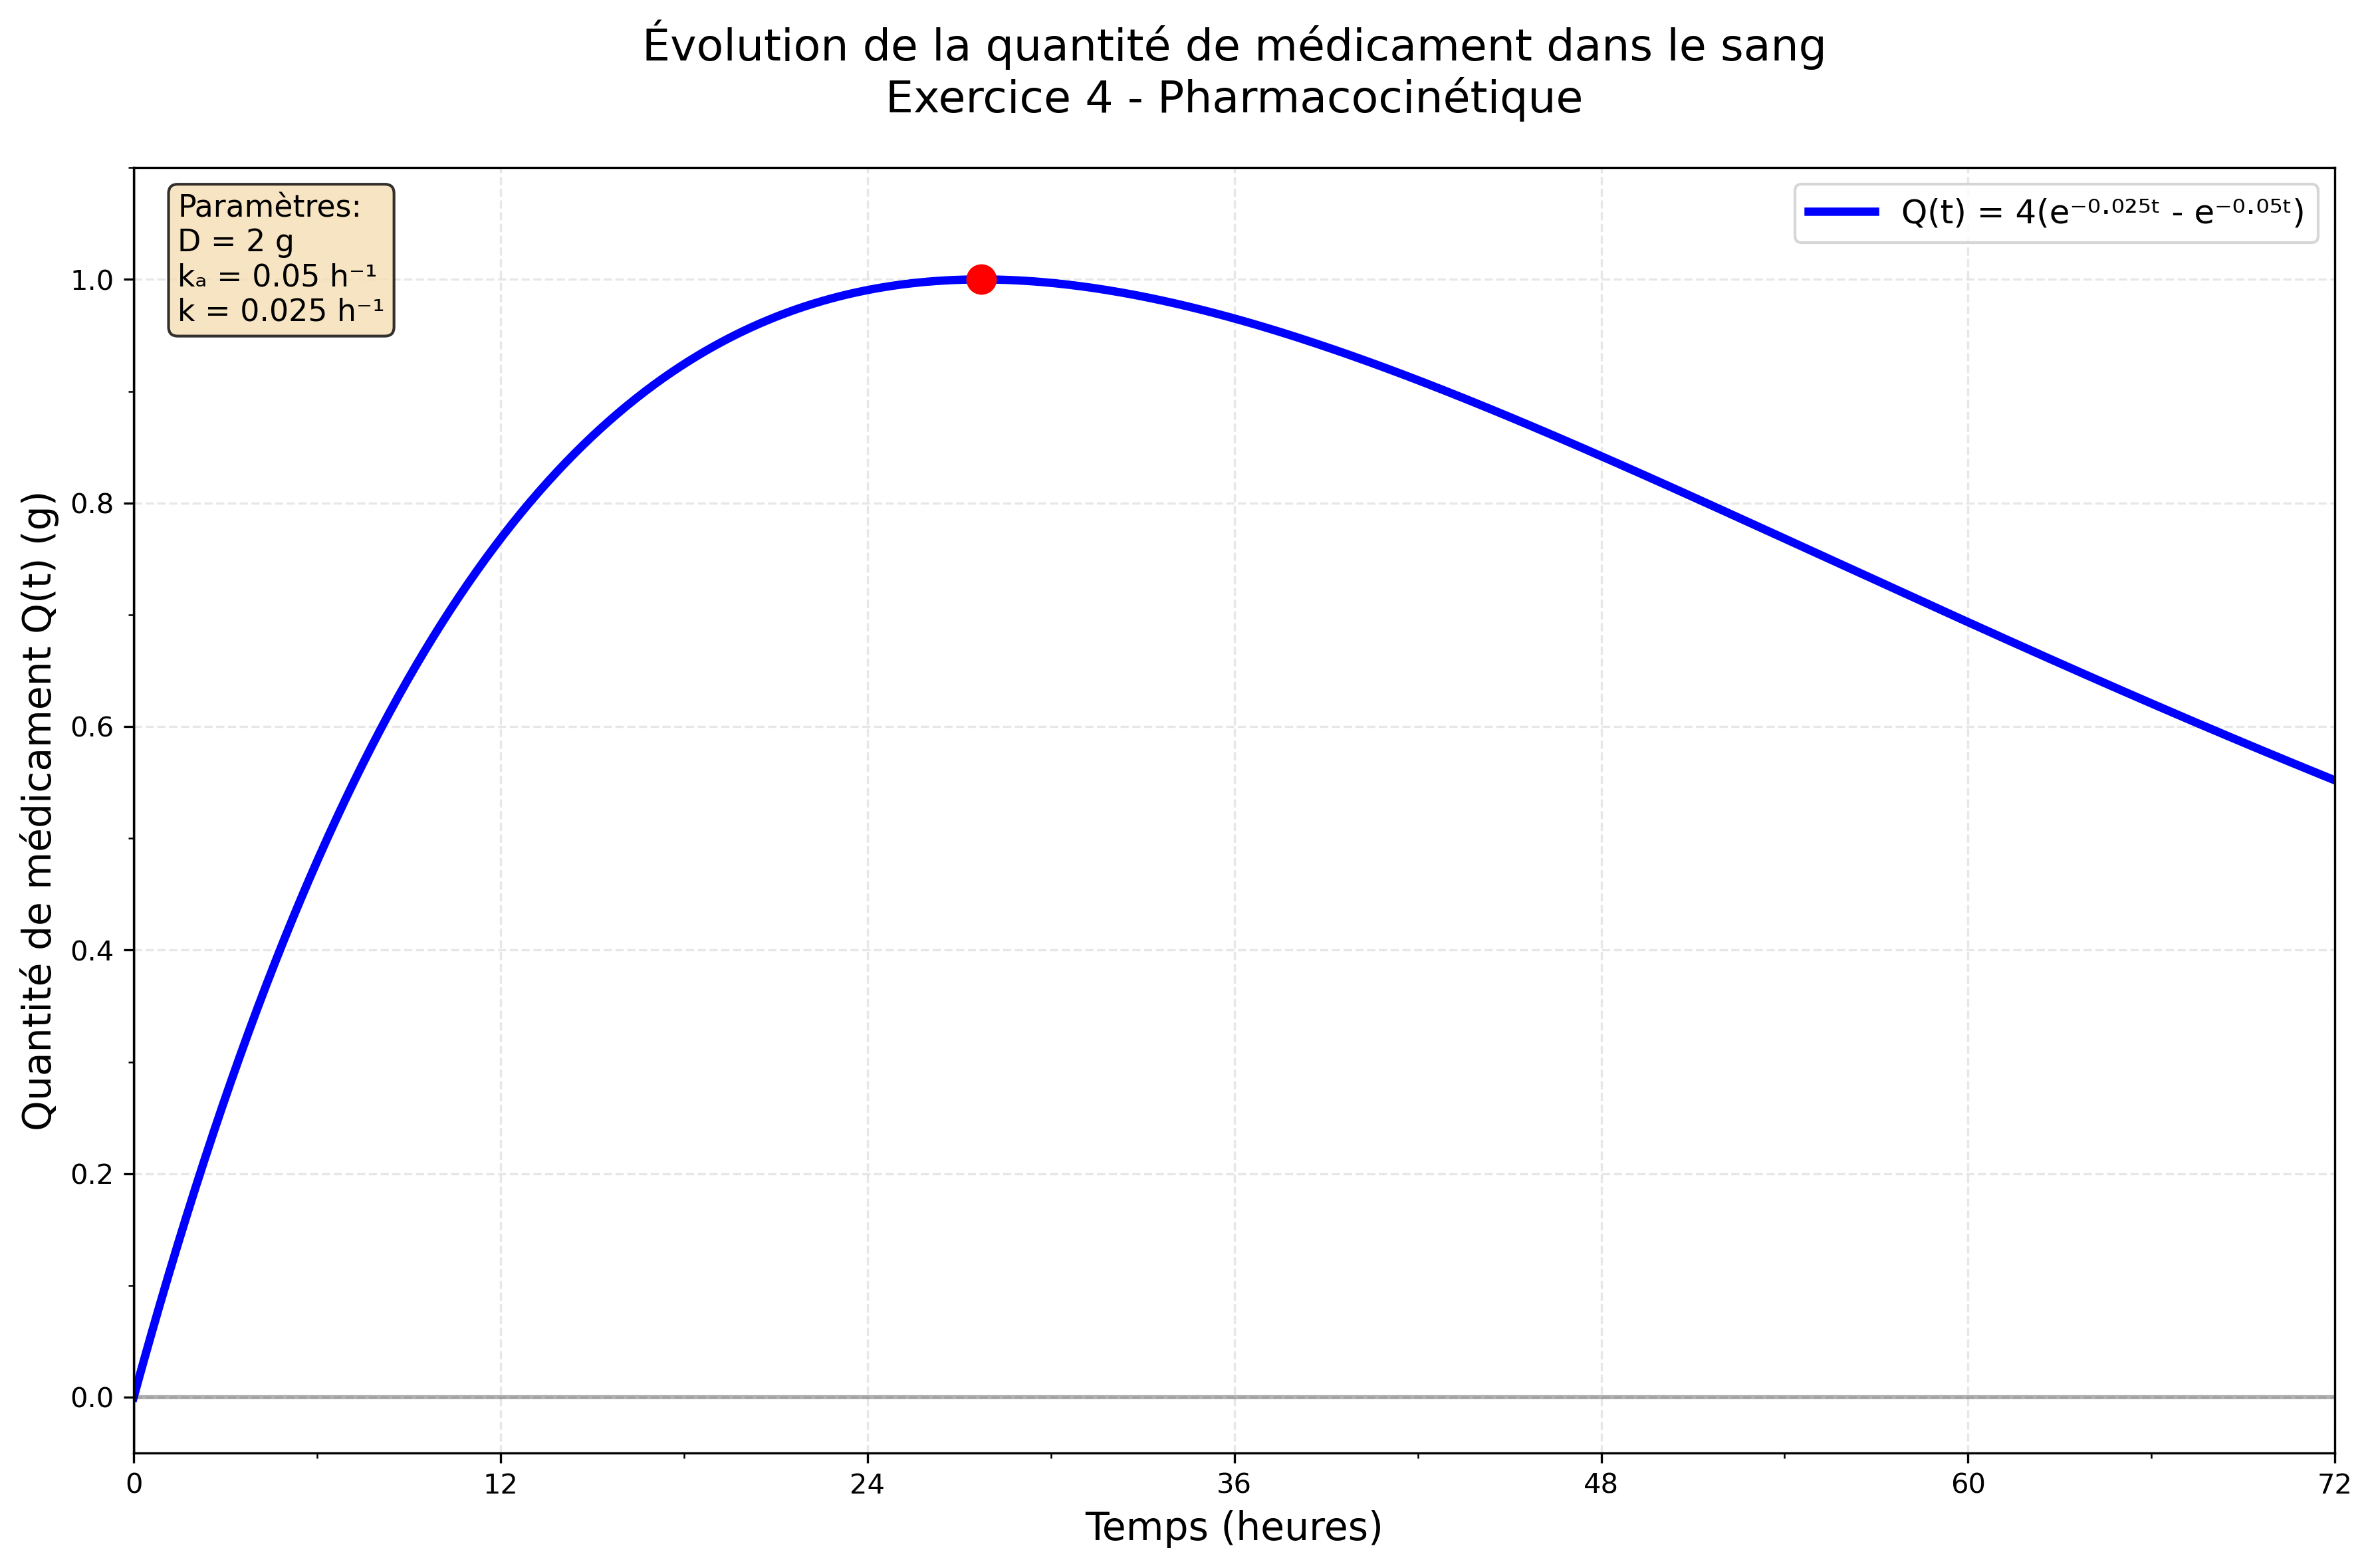
\includegraphics[width=0.6\textwidth]{images/courbe_pharmacocinetique.png}
\end{center}
\end{boitecorrige}


\newpage
\section{EDO du second ordre : méthodes avancées}

\subsection*{Exercice 16 - EDO du 2\textsuperscript{e} ordre : solution générale complète \niveau{\moyen}}

\begin{boiteexercice}
Résoudre les équations différentielles suivantes en trouvant la solution homogène et une solution particulière :
\begin{enumerate}[label=(\alph*)]
  \item $y'' + 3y' + 2y = 6\e^x$
  \item $y'' - 4y' + 4y = \e^{2x}$ (racine double au second membre)
  \item $y'' + 4y = 8\cos(2x)$ (résonance en cosinus)
  \item $y'' + 2y' + 5y = 10x\e^{-x}$ avec $y(0)=0$, $y'(0)=1$
\end{enumerate}
\end{boiteexercice}

\begin{boitecorrige}
\textbf{(a)} Équation caractéristique : $r^2+3r+2 = (r+1)(r+2) = 0$, racines $r_1=-1$, $r_2=-2$. Solution homogène : $y_h = C_1\e^{-x}+C_2\e^{-2x}$. Solution particulière $y_p = A\e^x$ (1 n'est pas racine) : $A+3A+2A = 6$, $A=1$.
\[
y = C_1\e^{-x} + C_2\e^{-2x} + \e^x
\]

\textbf{(b)} Racine double $r=2$. Solution homogène : $y_h = (C_1+C_2 x)\e^{2x}$.
Comme $r=2$ est racine double, on multiplie par $x^2$ : $y_p = Ax^2\e^{2x}$.
On calcule $y_p'' - 4y_p' + 4y_p = 2A\e^{2x} = \e^{2x}$, donc $A=1/2$.
\[
y = (C_1+C_2 x)\e^{2x} + \frac{x^2}{2}\e^{2x}
\]

\textbf{(c)} Homogène : $y_h = C_1\cos(2x)+C_2\sin(2x)$. Résonance : $y_p = x(A\cos(2x)+B\sin(2x))$.
On calcule $y_p''+4y_p = -4A\sin(2x)+4B\cos(2x) = 8\cos(2x)$, d'où $B=2$, $A=0$.
\[
y = C_1\cos(2x)+C_2\sin(2x)+2x\sin(2x)
\]

\textbf{(d)} Équation caractéristique : $r^2+2r+5=0$, racines $r=-1\pm 2j$. Solution homogène : $y_h = \e^{-x}(C_1\cos 2x+C_2\sin 2x)$. Solution particulière $y_p = \e^{-x}(Ax+B)$. On substitue : $y_p = \e^{-x}(Ax+B)$, $y_p' = \e^{-x}(A-Ax-B)$, $y_p'' = \e^{-x}(-2A+Ax+B)$. Donc $y_p''+2y_p'+5y_p = \e^{-x}(5Ax+5B) = 10x\e^{-x}$ : $A=2$, $B=0$.

Conditions initiales : $y(0) = C_1 = 0$, $y'(0) = -C_1+2C_2+2 = 1$, $C_2=-1/2$.
\[
y(x) = \e^{-x}\!\left(-\frac{1}{2}\sin 2x + 2x\right)
\]
\end{boitecorrige}

\subsection*{Exercice 17 - Variation des constantes pour $y'' + y = 1/\sin x$ \niveau{\difficile}}

\begin{boiteexercice}
Résoudre par la méthode de variation des constantes :
\[
y'' + y = \frac{1}{\sin x}, \quad x\in\,]0,\pi[
\]
\begin{enumerate}
  \item Trouver les deux solutions de l'équation homogène $y_1$ et $y_2$.
  \item Calculer le wronskien $W(y_1,y_2)$.
  \item Poser $y_p = C_1(x)y_1 + C_2(x)y_2$ et écrire le système pour $C_1'$ et $C_2'$.
  \item Intégrer et donner la solution particulière.
  \item Donner la solution générale.
\end{enumerate}
\end{boiteexercice}

\begin{boitecorrige}
\textbf{1.} L'équation homogène $y''+y=0$ a les racines $r=\pm j$ : $y_1 = \cos x$, $y_2 = \sin x$.

\textbf{2.} Wronskien : $W = y_1 y_2' - y_1' y_2 = \cos x\cos x - (-\sin x)\sin x = \cos^2 x + \sin^2 x = 1$.

\textbf{3.} Le système de variation des constantes est :
\[
C_1' y_1 + C_2' y_2 = 0, \quad C_1' y_1' + C_2' y_2' = \frac{1}{\sin x}
\]
D'où :
\[
C_1' = -\frac{y_2 f}{W} = -\frac{\sin x/\sin x}{1} = -1, \quad C_2' = \frac{y_1 f}{W} = \frac{\cos x/\sin x}{1} = \frac{\cos x}{\sin x}
\]

\textbf{4.} En intégrant :
\[
C_1 = -x, \quad C_2 = \int\frac{\cos x}{\sin x}\,\d x = \ln|\sin x| = \ln(\sin x) \quad\text{(car $x\in]0,\pi[$)}
\]
Solution particulière :
\[
y_p = -x\cos x + \sin x\ln(\sin x)
\]

\textbf{5.} Solution générale :
\[
\boxed{y = C_1\cos x + C_2\sin x - x\cos x + \sin x\ln(\sin x)}
\]
\end{boitecorrige}

\subsection*{Exercice 18 - Équation de Bessel d'ordre $n$ \niveau{\difficile}}

\begin{boiteexercice}
L'équation de Bessel d'ordre $n$ est :
\[
x^2 y'' + xy' + (x^2 - n^2)y = 0, \quad x > 0
\]
\begin{enumerate}
  \item Pour $n=0$, vérifier que la solution en série entière de la forme $y = \sum_{k=0}^\infty a_k x^{2k}$ ($a_0=1$) converge et calculer $a_1$ et $a_2$.
  \item On admet que les solutions régulières sont les fonctions de Bessel $J_n(x)$. Donner les premiers termes de $J_0(x)$ et $J_1(x)$.
  \item Pour le problème des modes propres d'une membrane circulaire de rayon $R$ (équation $\Delta u + k^2 u = 0$), les modes axiaux vérifient $J_0(k_{0n}R) = 0$. Calculer les 3 premiers zéros de $J_0$.
  \item La relation de récurrence $J_{n-1}(x)+J_{n+1}(x) = \frac{2n}{x}J_n(x)$ permet de calculer $J_n$ pour tout $n$. Calculer $J_2(1)$ sachant que $J_0(1)\approx0{,}765$ et $J_1(1)\approx0{,}440$.
\end{enumerate}
\end{boiteexercice}

\begin{boitecorrige}
\textbf{1.} Pour $n=0$, en substituant $y = \sum a_k x^{2k}$ dans $xy''+(y'+xy) = 0$... en fait dans $x^2 y''+xy'+x^2 y=0$, terme par terme :
\[
\sum_{k=0}^\infty\bigl[2k(2k-1)a_k x^{2k} + 2ka_k x^{2k} + a_{k-1}x^{2k}\bigr] = 0
\]
soit $(2k)^2 a_k + a_{k-1} = 0$, d'où $a_k = -a_{k-1}/(4k^2)$.

\[
a_0 = 1,\quad a_1 = -\frac{1}{4},\quad a_2 = \frac{1}{64},\quad a_3 = -\frac{1}{2304},\ldots
\]

\textbf{2.} Fonctions de Bessel :
\[
J_0(x) = 1 - \frac{x^2}{4} + \frac{x^4}{64} - \ldots = \sum_{k=0}^\infty \frac{(-1)^k}{(k!)^2}\left(\frac{x}{2}\right)^{2k}
\]
\[
J_1(x) = \frac{x}{2} - \frac{x^3}{16} + \ldots = \sum_{k=0}^\infty \frac{(-1)^k}{k!(k+1)!}\left(\frac{x}{2}\right)^{2k+1}
\]

\textbf{3.} Les trois premiers zéros de $J_0$ (tables) :
\[
z_{01}\approx 2{,}405,\quad z_{02}\approx 5{,}520,\quad z_{03}\approx 8{,}654
\]
Les fréquences propres sont $f_{0n} = c\, z_{0n}/(2\pi R)$ pour une membrane de rayon $R$.

\textbf{4.} Relation de récurrence pour $n=1$ :
\[
J_0(1) + J_2(1) = \frac{2}{1}J_1(1) \implies J_2(1) = 2J_1(1) - J_0(1)\approx 2\times0{,}440 - 0{,}765 = 0{,}115
\]
\end{boitecorrige}

\subsection*{Exercice 19 - Système d'EDO linéaire : résolution par valeurs propres \niveau{\difficile}}

\begin{boiteexercice}
On considère le système différentiel $\dot{X} = AX$ avec :
\[
A = \begin{pmatrix}0 & 1 \\ -2 & -3\end{pmatrix}
\]
\begin{enumerate}
  \item Calculer les valeurs propres et les vecteurs propres de $A$.
  \item En déduire la solution générale du système homogène.
  \item Résoudre le problème de Cauchy avec $X(0) = \begin{pmatrix}1\\0\end{pmatrix}$.
  \item Calculer l'exponentielle de matrice $\e^{At}$ et vérifier que $X(t) = \e^{At}X(0)$.
  \item Étudier le comportement asymptotique : vers quel état le système tend-il pour $t\to+\infty$ ?
\end{enumerate}
\end{boiteexercice}

\begin{boitecorrige}
\textbf{1.} Équation caractéristique : $\lambda^2+3\lambda+2 = (\lambda+1)(\lambda+2) = 0$, d'où $\lambda_1=-1$ et $\lambda_2=-2$.

Vecteur propre pour $\lambda_1=-1$ : $(A+I)v_1 = 0$ donne $\begin{pmatrix}1&1\\-2&-2\end{pmatrix}v_1=0$, soit $v_1 = \begin{pmatrix}1\\-1\end{pmatrix}$.

Vecteur propre pour $\lambda_2=-2$ : $(A+2I)v_2 = 0$ donne $v_2 = \begin{pmatrix}1\\-2\end{pmatrix}$.

\textbf{2.} Solution générale :
\[
X(t) = C_1\begin{pmatrix}1\\-1\end{pmatrix}\e^{-t} + C_2\begin{pmatrix}1\\-2\end{pmatrix}\e^{-2t}
\]

\textbf{3.} Conditions initiales $X(0) = \begin{pmatrix}1\\0\end{pmatrix}$ :
\[
C_1+C_2 = 1, \quad -C_1-2C_2 = 0 \implies C_1 = 2,\; C_2 = -1
\]
\[
X(t) = \begin{pmatrix}2\e^{-t}-\e^{-2t}\\-2\e^{-t}+2\e^{-2t}\end{pmatrix}
\]

\textbf{4.} La matrice fondamentale est $\Phi(t) = \begin{pmatrix}\e^{-t}&\e^{-2t}\\-\e^{-t}&-2\e^{-2t}\end{pmatrix}$ et $\e^{At} = \Phi(t)\Phi(0)^{-1}$.

$\Phi(0)^{-1} = \begin{pmatrix}2&1\\-1&-1\end{pmatrix}$, donc :
\[
\e^{At} = \begin{pmatrix}2\e^{-t}-\e^{-2t} & \e^{-t}-\e^{-2t}\\-2\e^{-t}+2\e^{-2t} & -\e^{-t}+2\e^{-2t}\end{pmatrix}
\]

\textbf{5.} Pour $t\to+\infty$ : les deux valeurs propres sont négatives ($\lambda_1=-1$, $\lambda_2=-2$), donc $X(t)\to\vec{0}$. L'origine est un \textbf{n\oe{}ud stable} : toutes les trajectoires convergent vers l'équilibre $X=0$.
\end{boitecorrige}

\subsection*{Exercice 20 - Équation de Legendre et polynômes de Legendre \niveau{\difficile}}

\begin{boiteexercice}
L'équation de Legendre est :
\[
(1-x^2)y'' - 2xy' + n(n+1)y = 0, \quad x\in[-1,1]
\]
\begin{enumerate}
  \item Montrer que $x=0$ est un point ordinaire et chercher une solution en série $y = \sum_{k=0}^\infty a_k x^k$.
  \item Montrer que les coefficients vérifient $a_{k+2} = -\frac{(n-k)(n+k+1)}{(k+2)(k+1)}a_k$.
  \item Pour $n=2$, en partant de $a_0=1$, $a_1=0$, calculer $P_2(x)$.
  \item Vérifier que $P_2(x) = \frac{1}{2}(3x^2-1)$ est bien solution.
  \item La condition d'orthogonalité est $\int_{-1}^1 P_m(x)P_n(x)\,\d x = \frac{2}{2n+1}\delta_{mn}$. Vérifier pour $m=0$, $n=2$.
\end{enumerate}
\end{boiteexercice}

\begin{boitecorrige}
\textbf{1.} En $x=0$, les coefficients sont $p(x)=-2x/(1-x^2)$ et $q(x)=n(n+1)/(1-x^2)$, continus en $x=0$ : point ordinaire. En substituant $y = \sum a_k x^k$ dans l'équation :
\[
(1-x^2)\sum_{k=2}^\infty k(k-1)a_k x^{k-2} - 2x\sum_{k=1}^\infty ka_k x^{k-1} + n(n+1)\sum a_k x^k = 0
\]

\textbf{2.} En collectant les termes en $x^k$ :
\[
(k+2)(k+1)a_{k+2} - k(k-1)a_k - 2ka_k + n(n+1)a_k = 0
\]
\[
a_{k+2} = \frac{k(k+1)-n(n+1)}{(k+2)(k+1)}a_k = -\frac{(n-k)(n+k+1)}{(k+2)(k+1)}a_k
\]

\textbf{3.} Pour $n=2$, $a_0=1$, $a_1=0$ :
\[
a_2 = -\frac{(2-0)(2+1)}{2\cdot1}a_0 = -3, \quad a_4 = -\frac{(2-2)(2+3)}{4\cdot3}a_2 = 0
\]
Donc la série est finie : $y = 1 - 3x^2$. Le polynôme normalisé est $P_2(x) = \frac{1}{2}(3x^2-1)$ (avec $a_0 = -1/2$ pour la normalisation standard $P_n(1)=1$).

\textbf{4.} Vérification : $P_2 = \frac{3x^2-1}{2}$, $P_2' = 3x$, $P_2'' = 3$.
\[
(1-x^2)\cdot3 - 2x\cdot3x + 2\cdot3\cdot\frac{3x^2-1}{2} = 3-3x^2-6x^2+9x^2-3 = 0\quad
\]

\textbf{5.} $P_0(x)=1$ et $P_2(x) = \frac{3x^2-1}{2}$ :
\[
\int_{-1}^1 P_0 P_2\,\d x = \int_{-1}^1\frac{3x^2-1}{2}\,\d x = \frac{1}{2}\left[x^3-x\right]_{-1}^1 = \frac{1}{2}(1-1-(-1+1)) = 0 = \delta_{02}\quad
\]
\end{boitecorrige}

\subsection*{Exercice 21 - Transformation de Laplace pour les EDO \niveau{\moyen}}

\begin{boiteexercice}
Rappel : $\mathcal{L}\{y'\} = sY(s)-y(0)$, $\mathcal{L}\{y''\} = s^2Y(s)-sy(0)-y'(0)$, $\mathcal{L}\{\e^{at}\} = 1/(s-a)$.

Résoudre par la transformée de Laplace :
\begin{enumerate}
  \item $y''+y = \sin t$ avec $y(0)=0$, $y'(0)=0$.
  \item $y''+4y'+4y = \e^{-2t}$ avec $y(0)=0$, $y'(0)=1$.
  \item $y''-y = \e^t + 1$ avec $y(0)=0$, $y'(0)=0$.
\end{enumerate}
\end{boiteexercice}

\begin{boitecorrige}
\textbf{1.} Transformée : $(s^2+1)Y = \mathcal{L}\{\sin t\} = 1/(s^2+1)$, donc $Y = 1/(s^2+1)^2$.

Décomposition partielle : $\mathcal{L}^{-1}\{1/(s^2+1)^2\} = \frac{1}{2}(\sin t - t\cos t)$.
\[
\boxed{y = \frac{1}{2}(\sin t - t\cos t)}
\]

\textbf{2.} Transformée (conditions $y(0)=0$, $y'(0)=1$) :
\[
(s^2+4s+4)Y - 1 = \frac{1}{s+2}
\]
\[
Y = \frac{1}{(s+2)^2} + \frac{1}{(s+2)^3}
\]
Inversée : $\mathcal{L}^{-1}\{1/(s+2)^2\} = t\e^{-2t}$, $\mathcal{L}^{-1}\{1/(s+2)^3\} = \frac{t^2}{2}\e^{-2t}$.
\[
y = t\e^{-2t} + \frac{t^2}{2}\e^{-2t} = \left(t+\frac{t^2}{2}\right)\e^{-2t}
\]

\textbf{3.} Transformée :
\[
(s^2-1)Y = \frac{1}{s-1} + \frac{1}{s} = \frac{s+s-1}{s(s-1)}
\]
\[
Y = \frac{2s-1}{s(s-1)(s+1)(s-1)} = \frac{2s-1}{s(s-1)^2(s+1)}
\]
Par fractions partielles : $Y = \frac{1}{s} + \frac{A}{s-1} + \frac{B}{(s-1)^2} + \frac{C}{s+1}$.

$s=0$ : $\frac{-1}{1\cdot(-1)} = 1$. $s\to\infty$ : A+C+1=0. $s=-1$ : $C = \frac{-3}{(-2)^2} = -3/4$. $s=1$ : $B = 1/2$. $A = -1/4$.
\[
y(t) = 1 - \frac{1}{4}\e^t + \frac{t}{2}\e^t - \frac{3}{4}\e^{-t} = 1 + \frac{2t-1}{4}\e^t - \frac{3}{4}\e^{-t}
\]
\end{boitecorrige}

\subsection*{Exercice 22 - Système proie-prédateur (Lotka-Volterra) \niveau{\difficile}}

\begin{boiteexercice}
On considère le système différentiel de Lotka-Volterra décrivant l'évolution couplée des populations de proies $x(t)$ et de prédateurs $y(t)$ :
\[
\dot x = ax - bxy, \qquad \dot y = -cy + dxy
\]
avec $a, b, c, d > 0$.
\begin{enumerate}
  \item Interpréter physiquement chaque terme.
  \item Trouver les points d'équilibre.
  \item Montrer que la quantité $H(x,y) = dx - c\ln x + by - a\ln y$ est conservée.
  \item Décrire qualitativement les trajectoires dans le plan de phase.
\end{enumerate}
\end{boiteexercice}

\begin{boitecorrige}
\textbf{1.} $ax$ : croissance naturelle des proies. $-bxy$ : mortalité due aux prédateurs. $-cy$ : mortalité naturelle des prédateurs. $+dxy$ : croissance des prédateurs proportionnelle aux proies consommées.

\textbf{2.} Points d'équilibre ($\dot x = \dot y = 0$) :
\[
(x, y) = (0, 0) \quad\text{ou}\quad (x^*, y^*) = (c/d, a/b)
\]

\textbf{3.} Dérivons $H$ le long des trajectoires :
\[
\frac{\d H}{\d t} = d\dot x - c\frac{\dot x}{x} + b\dot y - a\frac{\dot y}{y}
= \dot x\!\left(d - \frac{c}{x}\right) + \dot y\!\left(b - \frac{a}{y}\right)
\]
\[
= (ax - bxy)\frac{dx-c}{x} + (-cy+dxy)\frac{by-a}{y} = (a-by)(dx-c) - (c-dx)(a-by) = 0
\]
Donc $H$ est conservée : les trajectoires sont des courbes de niveau de $H$.

\textbf{4.} Les trajectoires sont des courbes fermées autour du point d'équilibre non trivial $(c/d, a/b)$ : les populations oscillent périodiquement (cycles proie-prédateur). Quand les proies abondent, les prédateurs prolifèrent, puis les proies diminuent, entraînant le déclin des prédateurs, et le cycle recommence.
\reponse{Équilibre $(c/d, a/b)$ ; $H(x,y) = dx - c\ln x + by - a\ln y$ conservée ; trajectoires fermées.}
\end{boitecorrige}

\subsection*{Exercice 23 - Équation de la chaleur 1D par séparation des variables \niveau{\difficile}}

\begin{boiteexercice}
On cherche à résoudre l'équation de la chaleur sur $[0, L]$ :
\[
\frac{\partial u}{\partial t} = D\frac{\partial^2 u}{\partial x^2}, \qquad u(0,t) = u(L,t) = 0, \quad u(x, 0) = f(x)
\]
\begin{enumerate}
  \item Chercher des solutions de la forme $u(x,t) = X(x)T(t)$ et établir les équations séparées.
  \item Déterminer les modes spatiaux $X_n(x)$ et temporels $T_n(t)$.
  \item Donner la solution générale.
  \item Pour $f(x) = u_0\sin(\pi x/L)$, donner la solution explicite.
\end{enumerate}
\end{boiteexercice}

\begin{boitecorrige}
\textbf{1.} $X T' = D X'' T$ soit $T'/T = D X''/X = -\lambda D$ (constante). D'où :
\[
X'' + (\lambda/D) X = 0, \qquad T' + \lambda T = 0
\]
(avec $\lambda > 0$ pour avoir décroissance temporelle)

\textbf{2.} Conditions aux limites $X(0) = X(L) = 0$ imposent $\lambda_n = D(n\pi/L)^2$ :
\[
X_n(x) = \sin\!\left(\frac{n\pi x}{L}\right), \qquad T_n(t) = \e^{-n^2\pi^2 D t/L^2}
\]

\textbf{3.} Solution générale (série de Fourier) :
\[
u(x,t) = \sum_{n=1}^\infty b_n \sin\!\left(\frac{n\pi x}{L}\right) \e^{-n^2\pi^2 D t/L^2}
\]
avec $b_n = \dfrac{2}{L}\displaystyle\int_0^L f(x)\sin\!\left(\dfrac{n\pi x}{L}\right)\d x$.

\textbf{4.} Pour $f(x) = u_0\sin(\pi x/L)$ : un seul mode $b_1 = u_0$, tous les autres $b_n = 0$ ($n\geq 2$).
\[
u(x,t) = u_0\sin\!\left(\frac{\pi x}{L}\right)\e^{-\pi^2 D t/L^2}
\]
Le profil spatial est conservé, l'amplitude décroît en exponentielle, avec constante de temps
\[
\tau = \frac{L^2}{\pi^2 D}.
\]
\reponse{$u(x,t) = \sum b_n \sin(n\pi x/L)\e^{-n^2\pi^2 Dt/L^2}$}
\end{boitecorrige}

\subsection*{Exercice 24 - Méthode d'Euler pour $\dot y = y$ \niveau{\facile}}

\begin{boiteexercice}
On considère l'EDO $\dot y = y$ avec $y(0) = 1$. La solution exacte est $y(t) = \e^t$.
\begin{enumerate}
  \item Rappeler le schéma d'Euler explicite de pas $h$.
  \item Calculer $y_1, y_2, y_3$ pour $h = 0{,}1$.
  \item Comparer avec les valeurs exactes.
  \item Donner l'erreur relative à $t = 0{,}3$.
\end{enumerate}
\end{boiteexercice}

\begin{boitecorrige}
\textbf{1.} Schéma d'Euler explicite :
\[
y_{n+1} = y_n + h\,f(t_n, y_n) = y_n(1 + h)
\]
(puisque $f(t,y) = y$).

\textbf{2.} Avec $h = 0{,}1$, $y_0 = 1$ :
\[
y_1 = 1{,}1, \quad y_2 = 1{,}21, \quad y_3 = 1{,}331
\]

\textbf{3.} Valeurs exactes : $\e^{0{,}1} \approx 1{,}1052$, $\e^{0{,}2} \approx 1{,}2214$, $\e^{0{,}3} \approx 1{,}3499$.

\textbf{4.} Erreur relative à $t = 0{,}3$ :
\[
\varepsilon = \frac{|1{,}331 - 1{,}3499|}{1{,}3499} \approx 1{,}4\,\%
\]
L'erreur locale à chaque pas est $O(h^2)$, l'erreur globale est $O(h)$.
\reponse{$y_3 \approx 1{,}331$ vs $\e^{0{,}3} \approx 1{,}3499$ ; erreur relative $\approx 1{,}4\,\%$.}
\end{boitecorrige}

\subsection*{Exercice 25 - Stabilité d'un schéma numérique \niveau{\moyen}}

\begin{boiteexercice}
On résout $\dot y = -\lambda y$ ($\lambda > 0$) par Euler explicite avec pas $h$.
\begin{enumerate}
  \item Donner la relation de récurrence.
  \item Étudier la stabilité : pour quelle condition sur $h$ la solution numérique reste-t-elle bornée ?
  \item Application : pour $\lambda = 10$, quel pas maximal garantit la stabilité ?
  \item Comparer avec le schéma d'Euler implicite.
\end{enumerate}
\end{boiteexercice}

\begin{boitecorrige}
\textbf{1.} $y_{n+1} = y_n - h\lambda y_n = (1 - h\lambda)\,y_n$, soit $y_n = (1 - h\lambda)^n y_0$.

\textbf{2.} Stabilité : $|y_n|$ doit rester bornée quand $n\to\infty$, soit $|1 - h\lambda| \leq 1$ :
\[
-1 \leq 1 - h\lambda \leq 1 \iff 0 \leq h\lambda \leq 2
\]
Condition de stabilité : $\boxed{h \leq 2/\lambda}$.

\textbf{3.} Pour $\lambda = 10$ : $h_\text{max} = 2/10 = 0{,}2$. Au-delà, la solution numérique oscille et diverge.

\textbf{4.} Schéma implicite : $y_{n+1} = y_n - h\lambda y_{n+1}$, soit $y_{n+1} = \dfrac{y_n}{1 + h\lambda}$. Quel que soit $h > 0$, $|1/(1+h\lambda)| < 1$ : schéma \textbf{inconditionnellement stable}. C'est l'avantage principal des schémas implicites pour les équations raides.
\reponse{Euler explicite : $h \leq 2/\lambda$ ; pour $\lambda=10$, $h_\text{max} = 0{,}2$. Euler implicite : stable $\forall h > 0$.}
\end{boitecorrige}

\newpage
\section*{Galerie d'illustrations - Équations différentielles}

\begin{figure}[H]
\centering
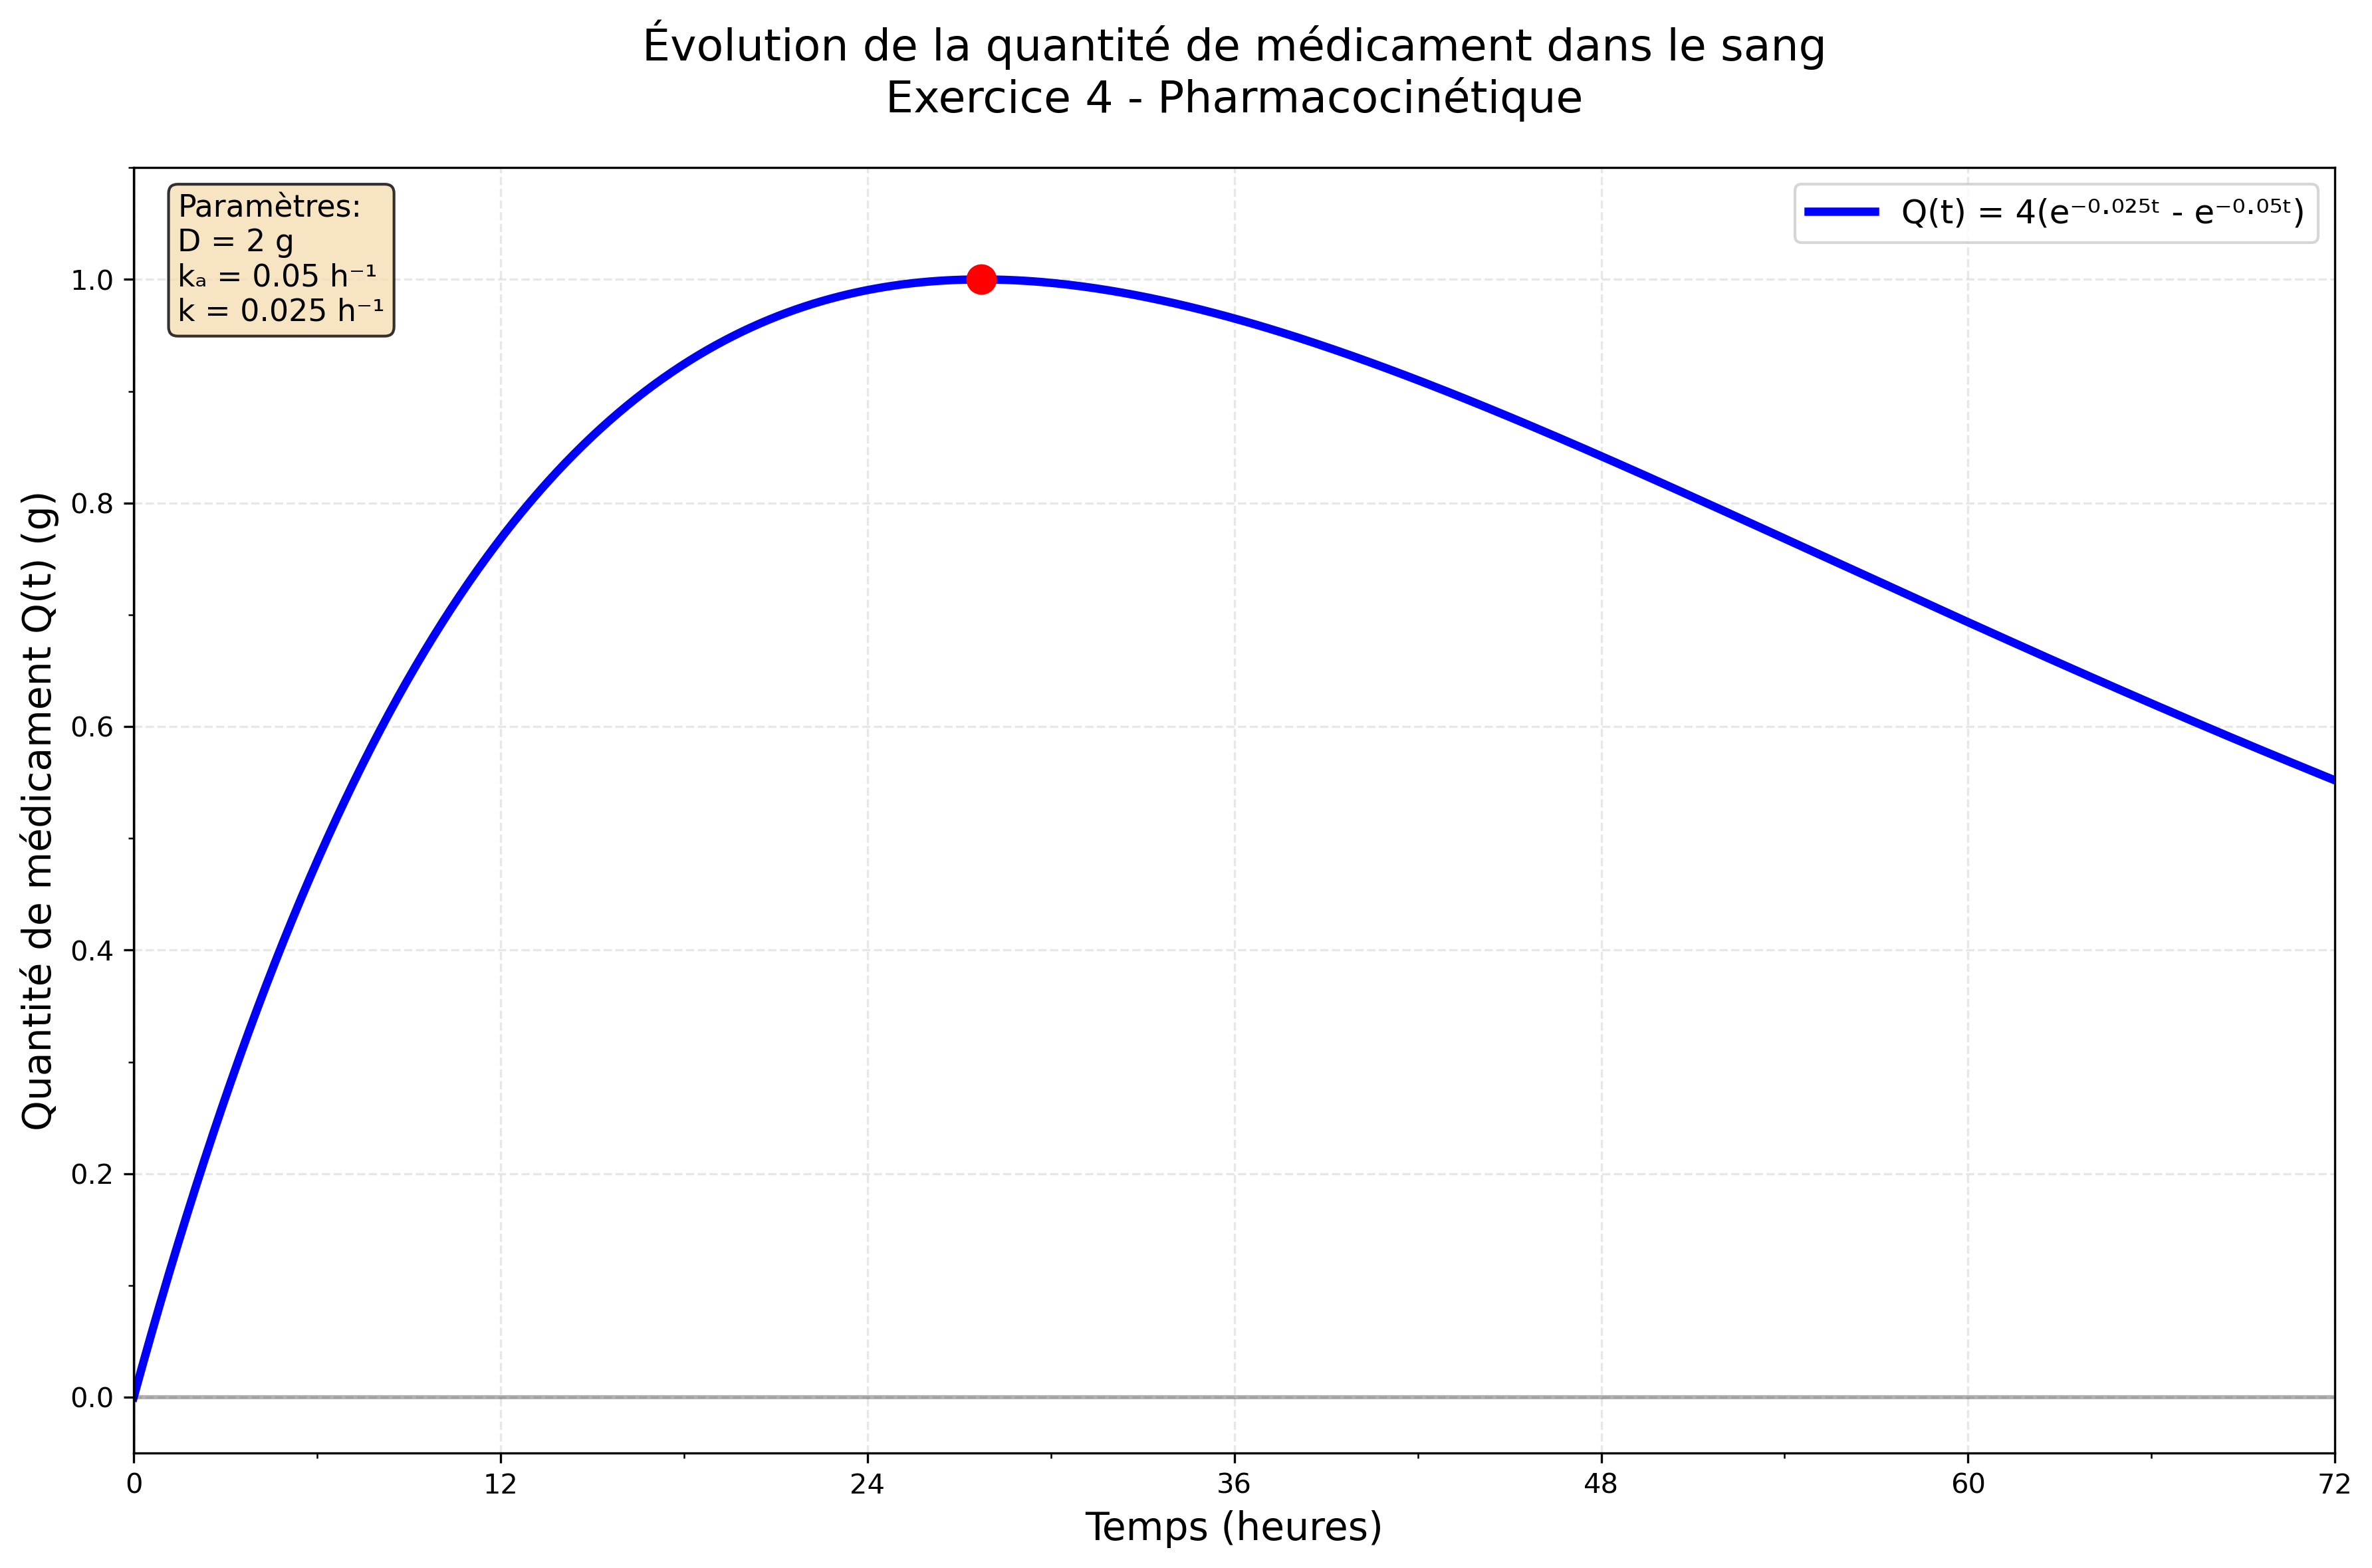
\includegraphics[width=0.7\textwidth]{images/edp/edo-028-000.png}
\caption{Résolution graphique d'une EDO.}
\end{figure}

\begin{figure}[H]
\centering

\includegraphics[width=0.7\textwidth]{images/edp/edo-028-001.png}
\caption{Champ de vecteurs et trajectoires.}
\end{figure}

\ifdefined\inMainDoc\else\end{document}\fi
